\section{Evaluation}
\label{sec:auswertung}

In this chapter the threshold current of the diode laser and the absorption spectrum of rubidium is evaluated. 

\subsection{Threshold Current}

As said in \autoref{sec:ThresholdCurrent} described the current is increased until the chip changes form the LED to laser operation.
The threshold current is detected at a laser current of $I_L = \SI{34.5}{\milli\ampere}$ at a cell temperature of $T_\text{cell} = \SI{49.9}{\celsius}$.
The LED mode can be seen in \autoref{fig:LED} and the laser mode in \autoref{fig:laser}. 
One can differentiate the different modes of the diode via the speckles on the IR Viewing Card.
These speckles occur then coherent light hits the IR Viewing Card. 
The IR Viewing Card is not a smooth surface and interference effects appear at the bumps at the surface, which results in the mention speckles.

\begin{figure}[H]
    \centering
    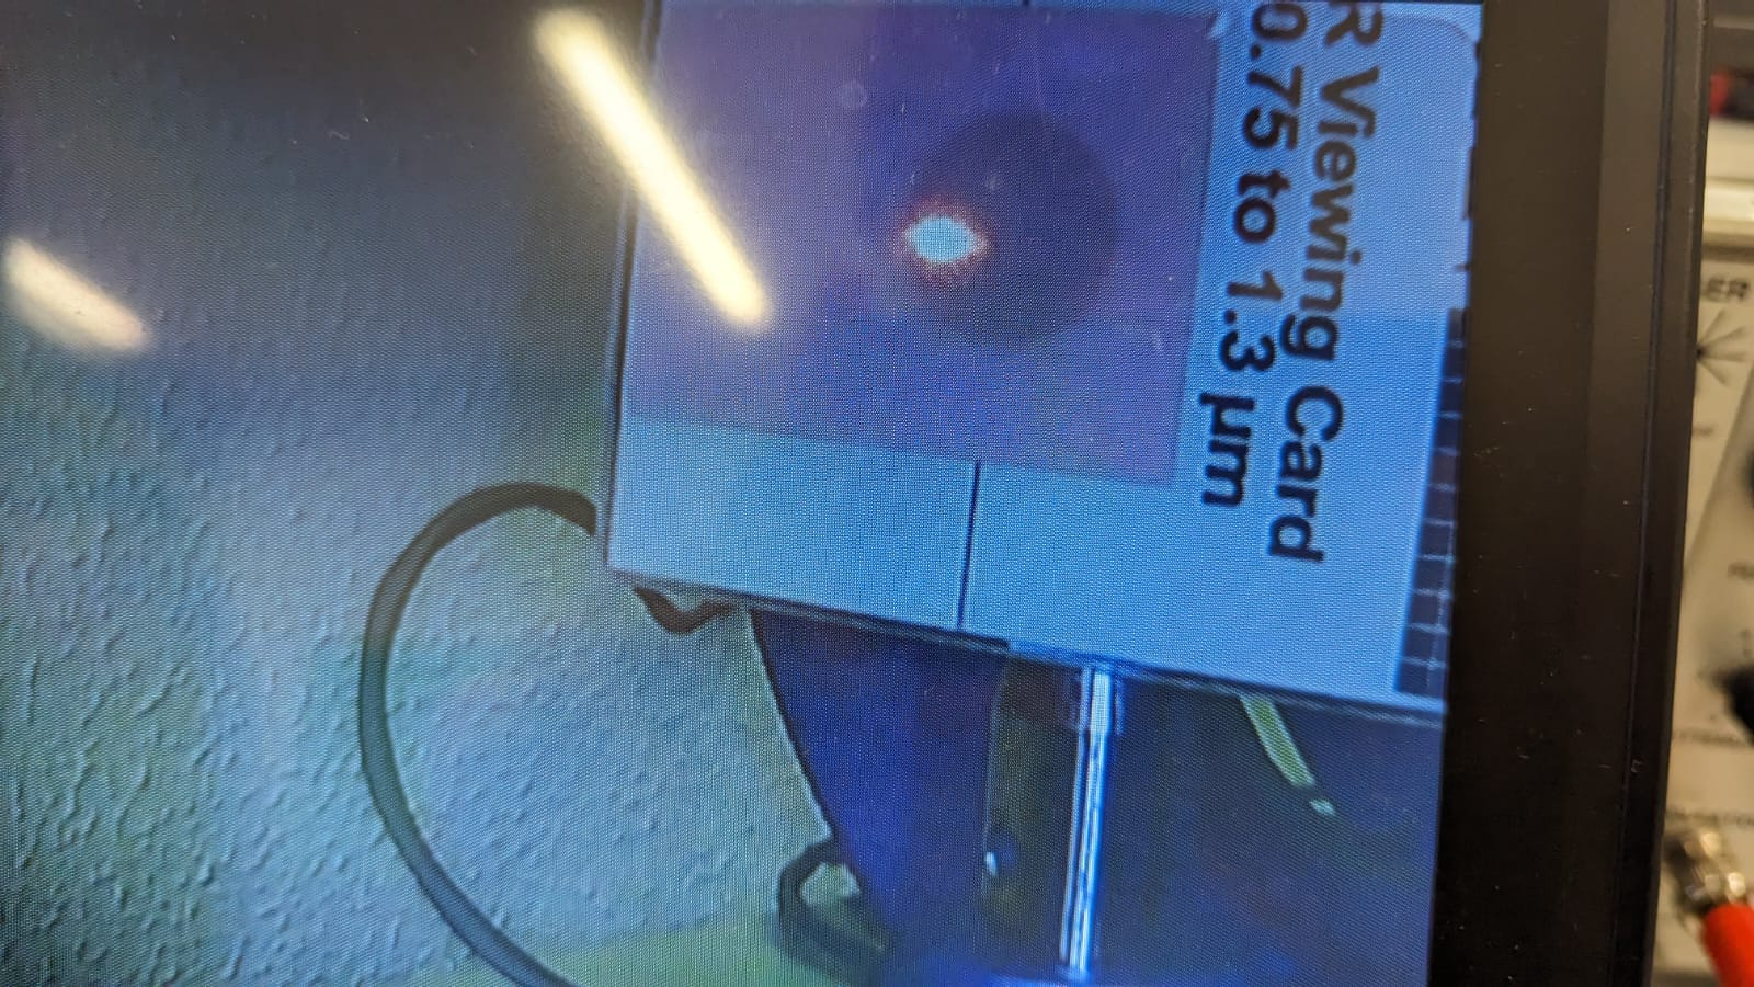
\includegraphics[width=\textwidth]{data/08.pdf}
    \caption{Photograph of the monitor, which is connected to the CCD Camera. The diode is in the LED mode.}
    \label{fig:LED}
\end{figure}

\begin{figure}[H]
    \centering
    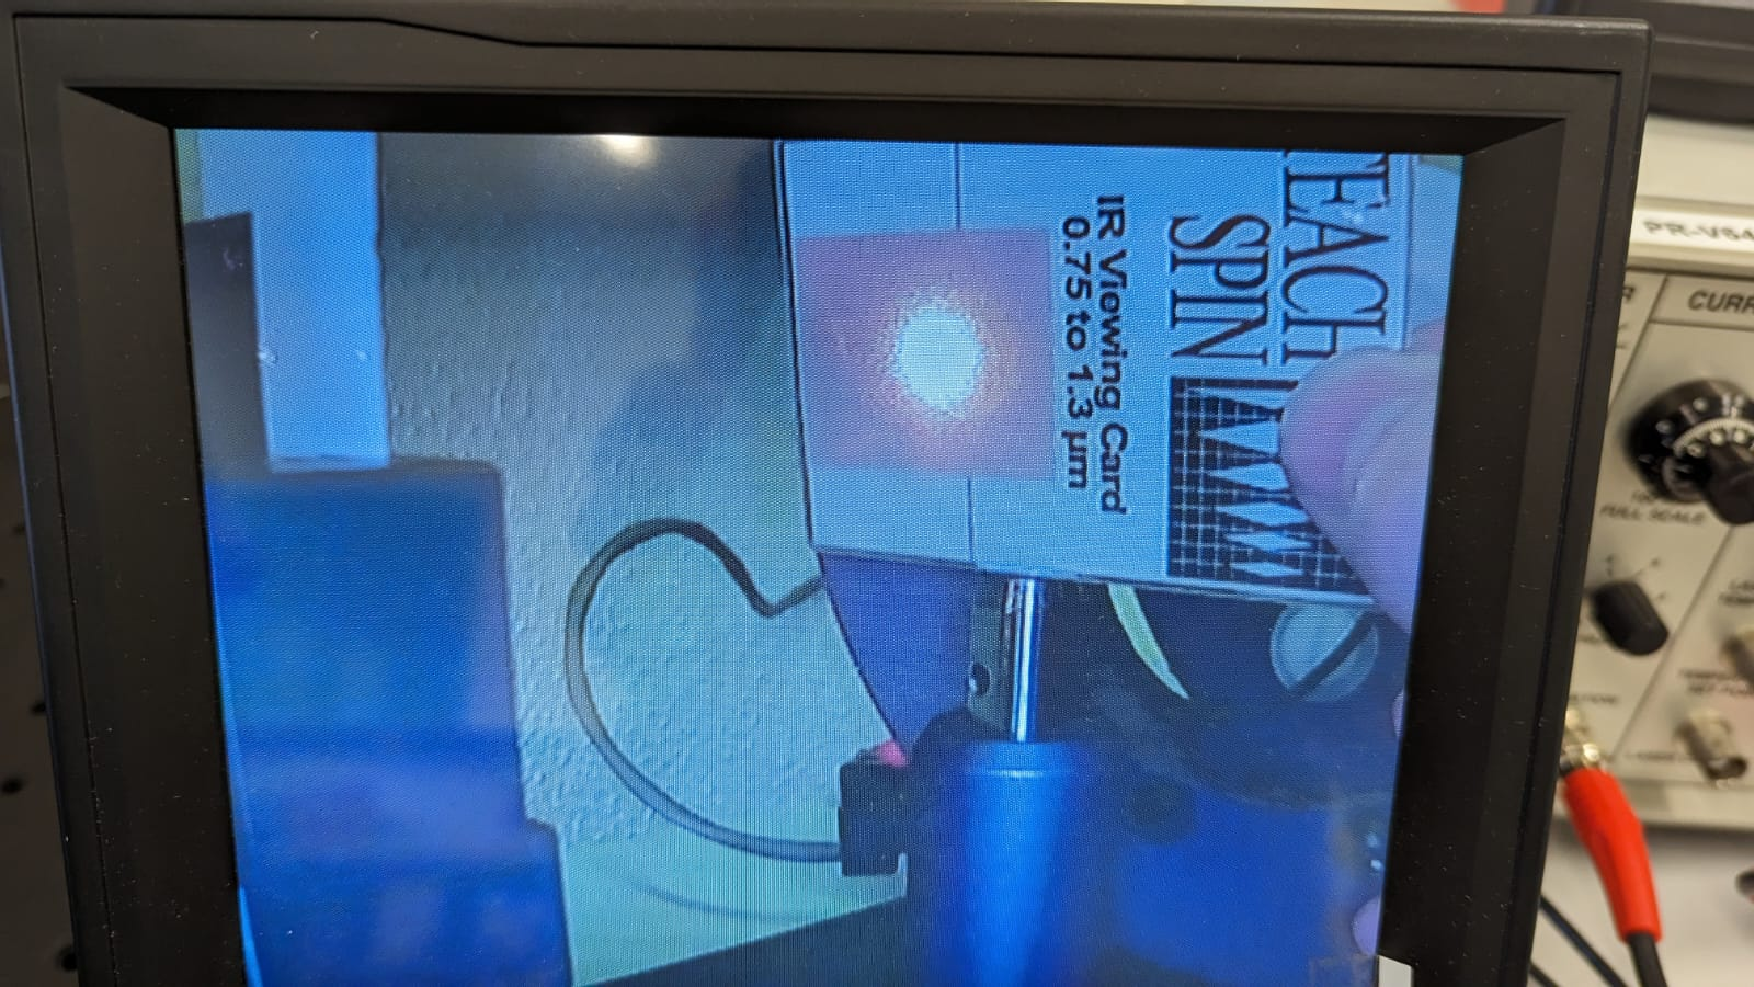
\includegraphics[width=\textwidth]{data/01.pdf}
    \caption{Photograph of the monitor, which is connected to the CCD Camera. The diode is in the laser mode.}
    \label{fig:laser}
\end{figure}


\subsection{Florescence and Trasmission Spectrum  of Rubidium}

The florescence of rubidium is depicted in \autoref{fig:florescence} and the absorption spectrum in \autoref{fig:Spectrum}.
The peaks can be identified as the transitions from left to right as 87b, 85b, 85a and 87a, if compared to \autoref{fig:rubidium}.

\begin{figure}[H]
    \centering
    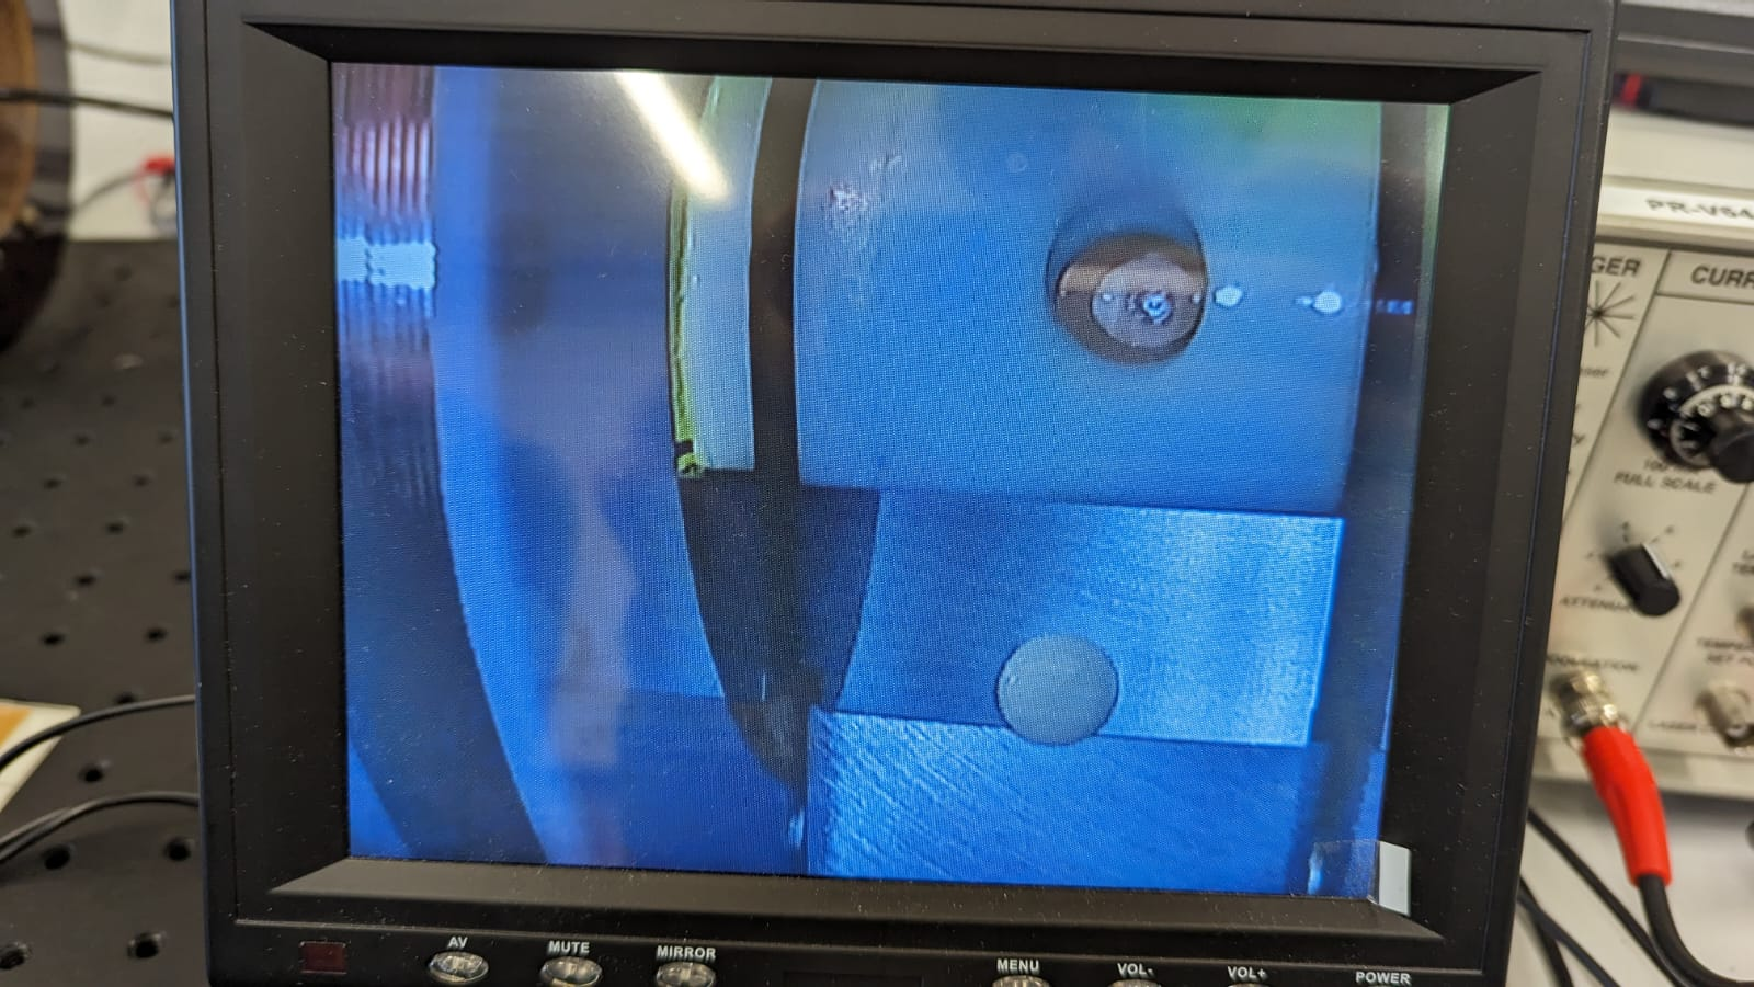
\includegraphics[width=\textwidth]{data/06.pdf}
    \caption{Florescence of rubidium.}
    \label{fig:florescence}
\end{figure}

\begin{figure}[H]
    \centering
    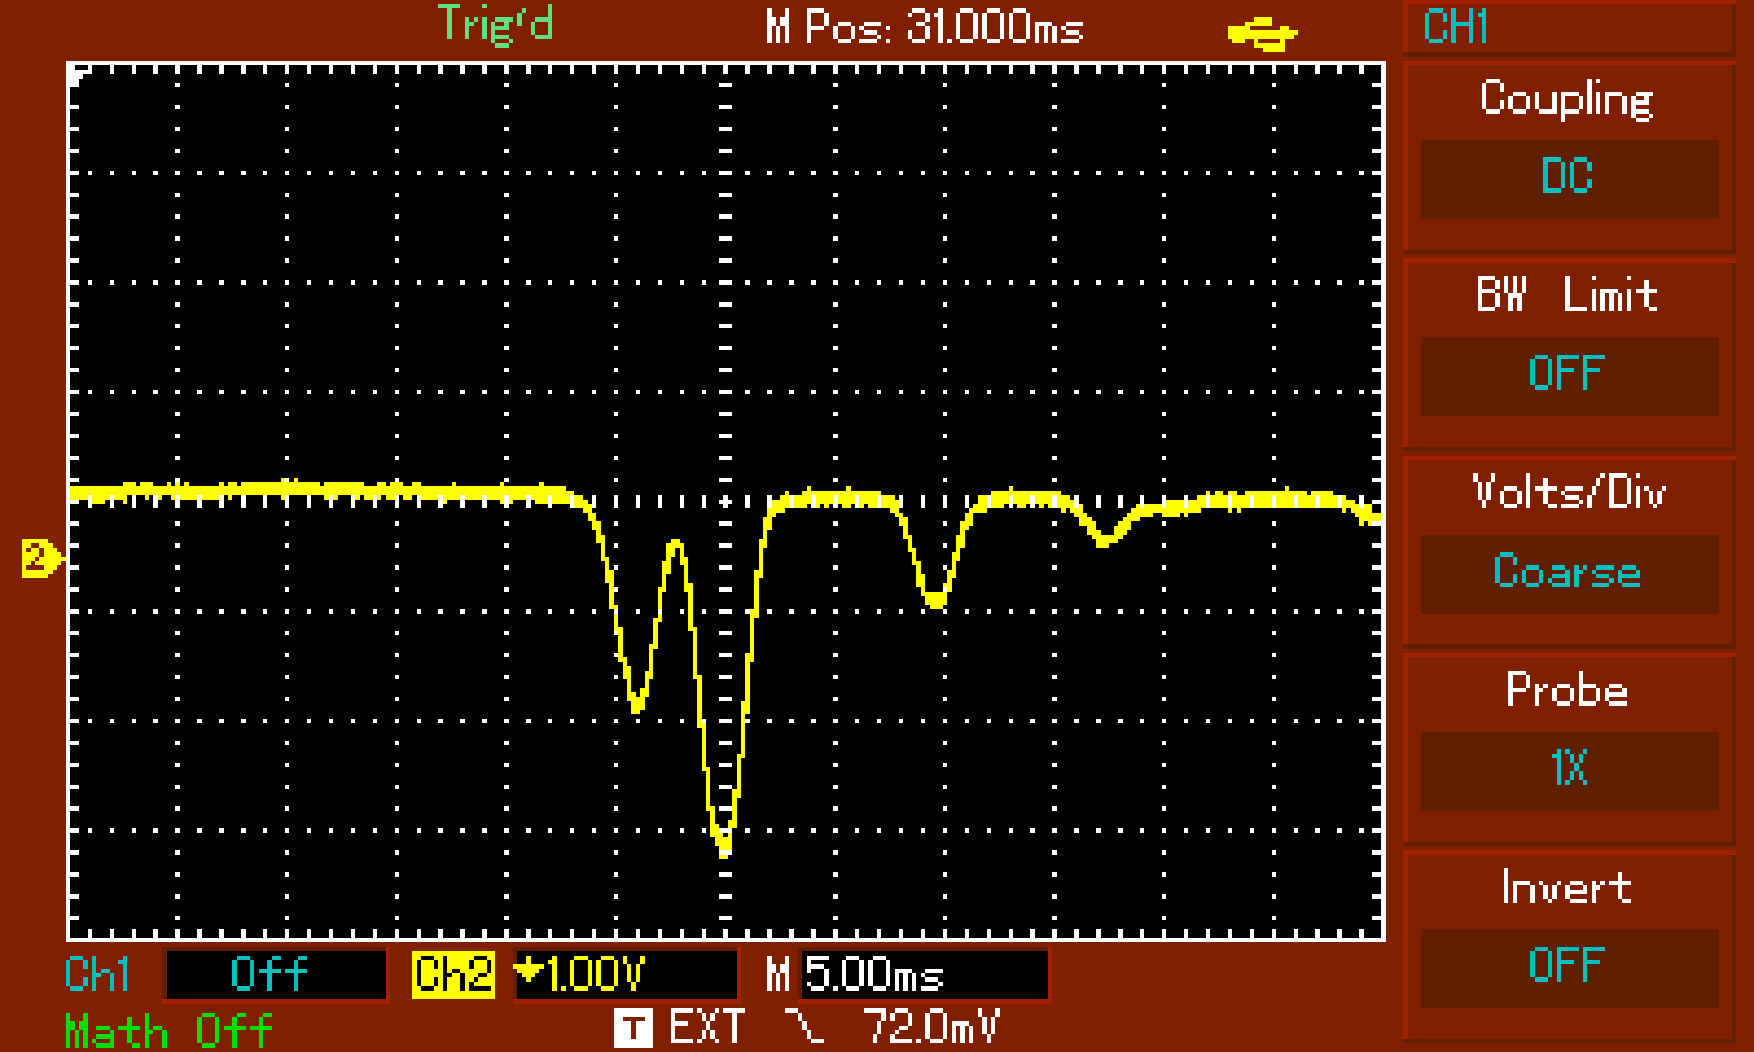
\includegraphics[width=\textwidth]{data/5.pdf}
    \caption{Picture of the oscilloscope showing the absorption spectrum of rubidium.}
    \label{fig:Spectrum}
\end{figure}
